% Permission is granted to copy, distribute and/or modify this document
% under the terms of the GNU Free Documentation License, Version 1.2
% or any later version published by the Free Software Foundation;
% with no Invariant Sections, no Front-Cover Texts, and no Back-Cover
% Texts.  A copy of the license is included in the section entitled "GNU
% Free Documentation License".
% Copyright 2014 EDF
%


%%%%%%%%%%%%%%%%%%%%%%%%%%%%%%%%%%%%%%%%%%%%%%%%%%%%%%%%%%%%%%%%%%%%%%%%%%%%%%%%%%%%%%%%%%
\section{Validation}

This section aims at exposing the methodology used to validate numerical results of the module.

\subsection{Methodology of validation}

This module implements two different algorithms:
\begin{itemize}
\item Monte Carlo
\item Simulated annealing algorithm; this algorithm is the novelty and requires several steps.
It uses also some tips such as the update of criterion after a permutation instead of a complete calculation.
\end{itemize}

Both algorithms are to be validated.

\subsection{Preliminary validations}
For specific designs, criteria values ($C_2$, \textit{mindist} and $\phi_{p}$) obtained with \textit{otlhs} module are compared with values computed by the \texttt{DiceDesign} R package.
Those scripts are located in the \texttt{validation} folder of this module.  Comparisons are very good, absolute error is less than $10^{-13}$. \\

As mentionned previously, $C_2$ criterion can be computed efficiently when a small perturbation is performed on design.
This specific method is compared to the \texttt{DiceDesign}'s ones: absolute error is less or equal to $10^{-10}$.\\

Note that for $\phi_p$ criterion, \texttt{DiceDesign} computes the new value after a permutation without taking into account the oldest criterion.
In this module, criterion update has been implemented, but is used only when parameter $p \geq$ 5. Indeed, numerical experiments have shown instability of the update when $p$ becomes large.


\subsection{Validation of Monte Carlo algorithm}
To get an optimal design using Monte Carlo algorithm, several designs are to be generated and the returned one minimizes the space filling function.\\

As the evaluation of the criterion does not require any complexity, validation of Monte Carlo algorithm is trivial:
\begin{itemize}
 \item Fix a criterion to minimize;
 \item Fix the RandomSeed to a fixed value (0 for example);
 \item Generate $N=100$ designs: get the optimal one and the associated criterion value;
 \item Fix again the RandomSeed;
 \item Generate $N=10000$ designs: get the optimal one and its associated criterion value;
 \item Check that the last criterion value is less or equal than to the previous one;
\end{itemize}

\subsection{Validation of simulated annealing algorithm}

Simulated annealing is compared to Monte Carlo algorithm (with $N=10000$) and should return better results.
Indeed the optimal design is built such as the space filling criterion decreases at each iteration.\\

Several use cases are proposed for the validation and illustrated hereafter:

\begin{table}[!h]
\begin{tabular}{|c|c|c|c|c|c|}
 \hline
 Test id & Dimension & Size &  Temperature profile & Profile parameters & Requirement\\
 \hline
 1 & 2 & 10 & Geometric & $T_0=10, c=0.999, iMax=50000$ & $C_2 \leq 0.0664$ \\
 \hline
 2 & 2 & 10 & Linear & $T_0=10, iMax=50000$ & mindist $\geq 0.272$\\
 \hline
 3 & 50 & 100 & Geometric & $T_0=10, c=0.999, iMax=50000$ & $C_2 \leq 22.176$\\
 \hline
 4 & 50 & 100 & Geometric & $T_0=10, c=0.999, iMax=50000$ & mindist $\geq 2.653$\\
 \hline
\end{tabular}
\caption{Use cases for the validation \& requirements}
\label{validationcases}
\end{table}

Final criteria should meet requirements.

\subsection{Results}
Designs are generated according to the multivariate distribution $U[0,1]^d$.

\subsubsection{MonteCarlo results}

We first check that Monte Carlo scales linearly with respect to the number of simulations.
Random generator seed is reinitialized to the same value when starting Monte Carlo algorithm, this is why criterion always decreases.

\begin{figure}[!h]
\begin{center}
\begin{tabular}{cc}
 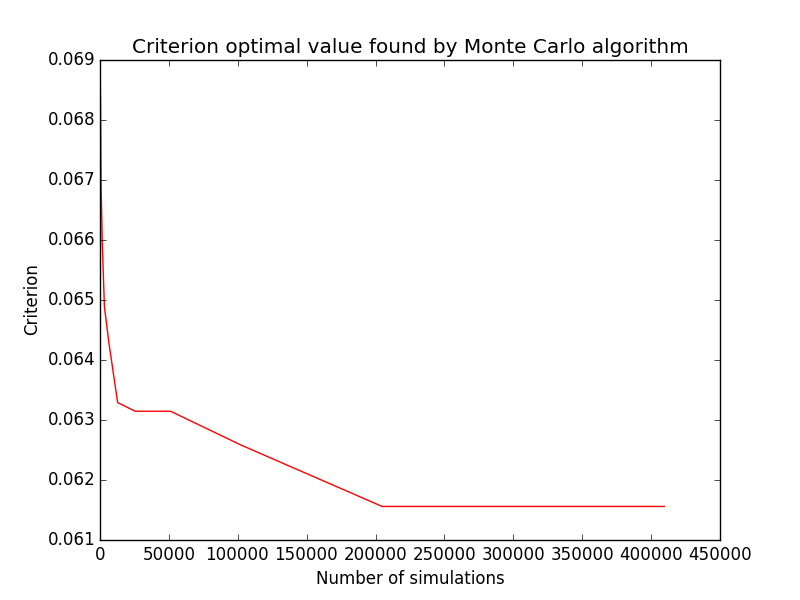
\includegraphics[scale=0.45]{lhs_mc_criterion.png} & 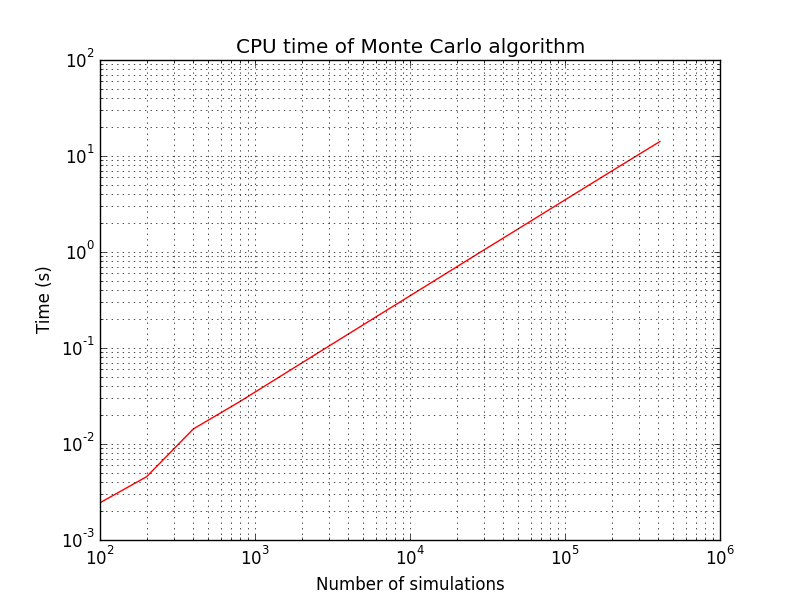
\includegraphics[scale=0.45]{lhs_mc_cpu_time.png}
\end{tabular}
\end{center}
\caption{Scaling of Monte Carlo results when increasing number of simulations}
\label{mc_scaling}
\end{figure}


Tests corresponding to use cases in table \ref{validationcases} are implemented and results obtained using Monte Carlo are given in table \ref{mc_validation_cases}.\\
\begin{table}[!h]
\begin{center}
\begin{tabular}{|c|c|c|c|c|c|}
 \hline
 Dimension & Size & Criterion & Criterion value & CPU time (s) & Requirement\\
 \hline
 2 & 10 & $C_2$ & 0.0643 & 0.72 & $C_2 \leq 0.0664$\\
 \hline
 2 & 10 & mindist & 0.2666 & 0.47 & mindist $\geq 0.272$\\
 \hline
 50 & 100 & $C_2$ & 24.427 & 109.48 & $C_2 \leq 22.176$\\
 \hline
 50 & 100 & mindist & 2.198 & 53.36 & mindist $\geq 2.653$\\
 \hline
\end{tabular}
\end{center}
\caption{Monte Carlo results after $N_{simu}=10000$ simulations}
\label{mc_validation_cases}
\end{table}

We use $N_{simu}=10000$ simulations in order to get the optimal design (designs are not centered).  As shown in figure~\ref{mc_scaling}, $10000$ iterations give a good solution for the small case; but it the larger case, it is expected that this number is way too small, so results are quite close to expectations.

In addition, we give design plots in dimension $2$ only (in dimension $50$, the interest is very limited).\\
\begin{figure}[!h]
\begin{center}
\begin{tabular}{cc}
 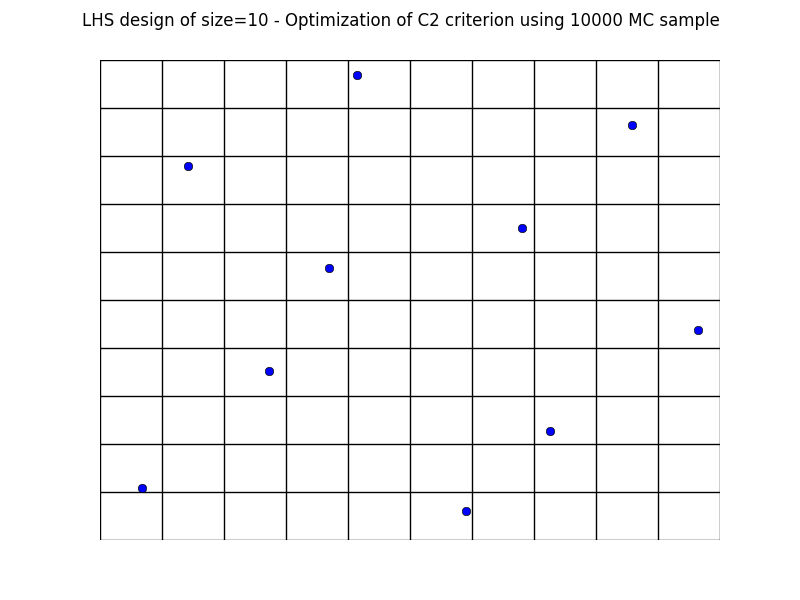
\includegraphics[scale=0.35]{lhs_mc_c2_10.png} & 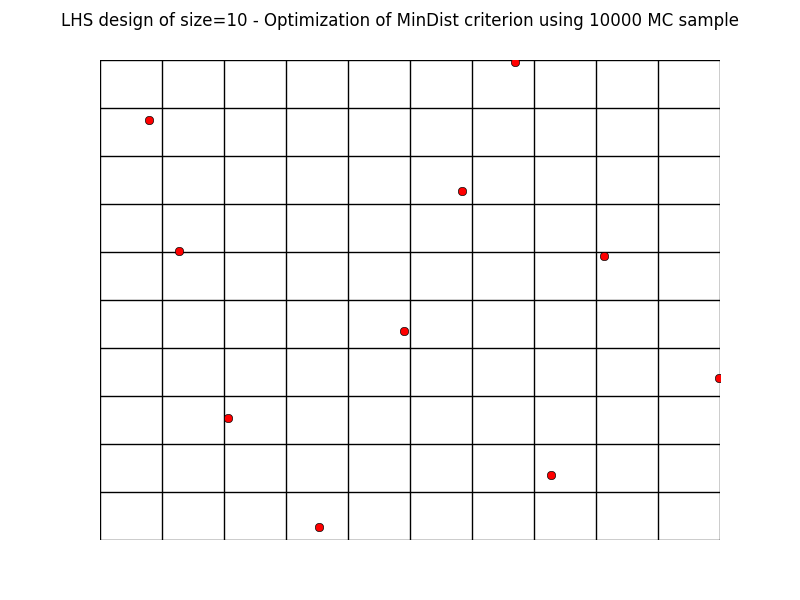
\includegraphics[scale=0.35]{lhs_mc_mindist_10.png}
\end{tabular}
\end{center}
\caption{Monte Carlo results}
\label{mc_graph_results}
\end{figure}


\subsubsection{Simulated annealing results}

Using the \texttt{SimulatedAnnealingLHS} class and use cases described in table \ref{validationcases}, tests are implemented and results are resumed in table \ref{results_module}.
These are compared to those produced by \texttt{DiceDesign} R package in terms of criteria and CPU time. 

\begin{table}[h]
\centering
\begin{tabular}{|c|c||c|c||c|c|}
 \hline
         &             & \multicolumn{2}{c||}{\texttt{otlhs}} & \multicolumn{2}{c|}{R} \\
\cline{3-6}
 Test id & Requirement & Criterion & CPU time (s) & Criterion & CPU time (s) \\
 \hline
 1 & $C_2 \leq 0.0664$ & $0.0699$ & $0.04$ & $0.06153$ & $89.8$\\
 \hline
 2 & mindist $\geq 0.272$ & $0.254$ & $0.246$ & $0.258$ & $36.37$\\
 \hline
 3 & $C_2 \leq 22.176$ & $22.190$ & $2.69$ & $22.15$& $618.7$ \\
 \hline
 4 & mindist $\geq 2.653$ & $2.643$ & $55.8$& $2.64$& $220.6$\\
 \hline
\end{tabular}
\caption{Numerical results obtained with the module}
\label{results_module}
\end{table}

CPU time is much lower with \textit{otlhs}.  It must be noted that speedup of
test~4 is not in par with speedups of other tests.  We believe that this is not
due to some performance problems, but is the combination of several factors:
\begin{enumerate}
\item R implementation of mindist is better than C2 because it does not contain loops, but only few high-level operations on matrices.
\item In \textit{otlhs} implementations, mindist is slower than C2 because it calls \texttt{evaluate} instead of \texttt{perturbLHS}.  It may be interesting to try with $p=5$ instead of $p=50$, mindist would then be as fast as C2, and many restarts could be tried.  Unfortunately, we did not have time to make these tests.
\end{enumerate}

Results are close to expectations, but do not meet all requirements.  In order to understand why \textit{otlhs} results are sometimes out of bounds, we performed 400~runs of tests~1 and~2 with DiceDesign and \textit{otlhs}, 40~runs of test~3 and 80~runs of test~4.
Results are shown in figure~\ref{comp_otlhs_dicedesign_tests}.
Diagrams look similar, thus in our opinion, \textit{otlhs} does meet requirements.  Moreover, as \textit{otlhs} is much faster than R, the same CPU budget will give better results with \textit{otlhs}.

\begin{figure}[!h]
\begin{center}
\begin{tabular}{cc}
 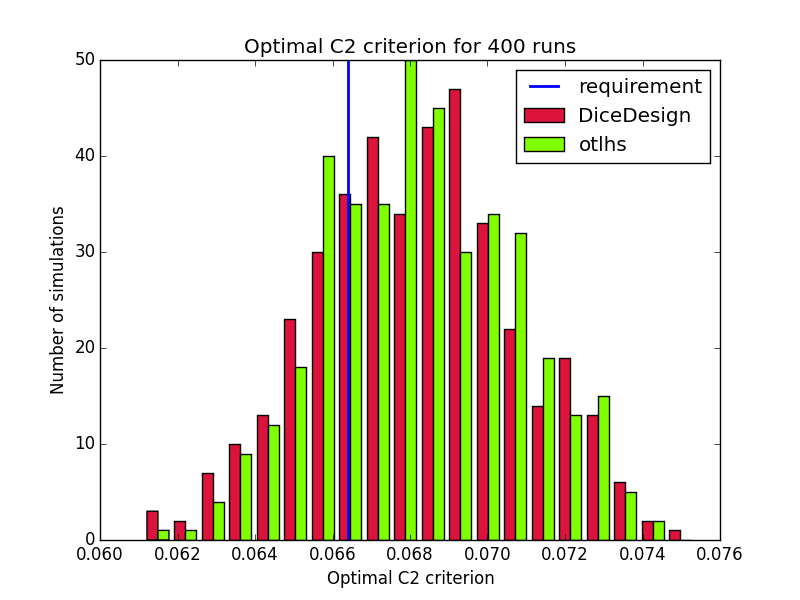
\includegraphics[scale=0.4]{comp_c2_small.png} & 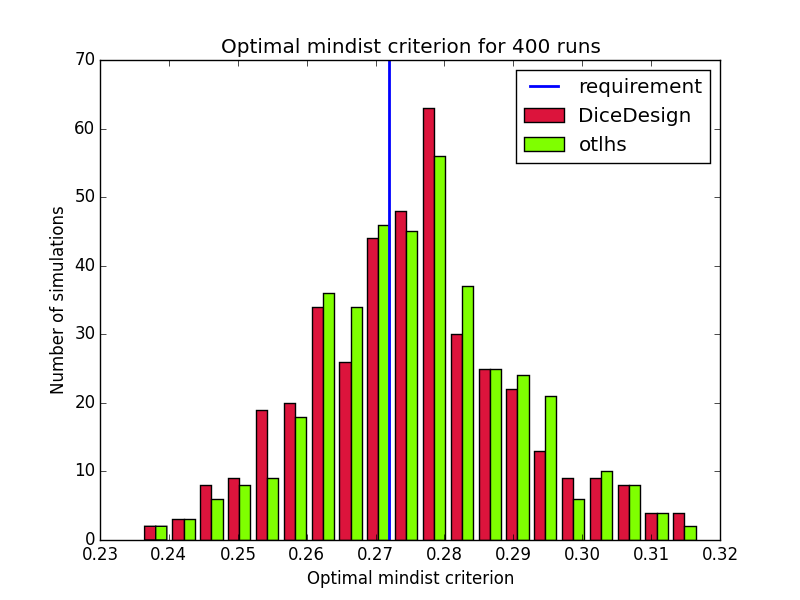
\includegraphics[scale=0.4]{comp_mindist_small.png}\\
 Comparison on 400 runs for test id 1 & Comparison on 400 runs for test id 2\\
 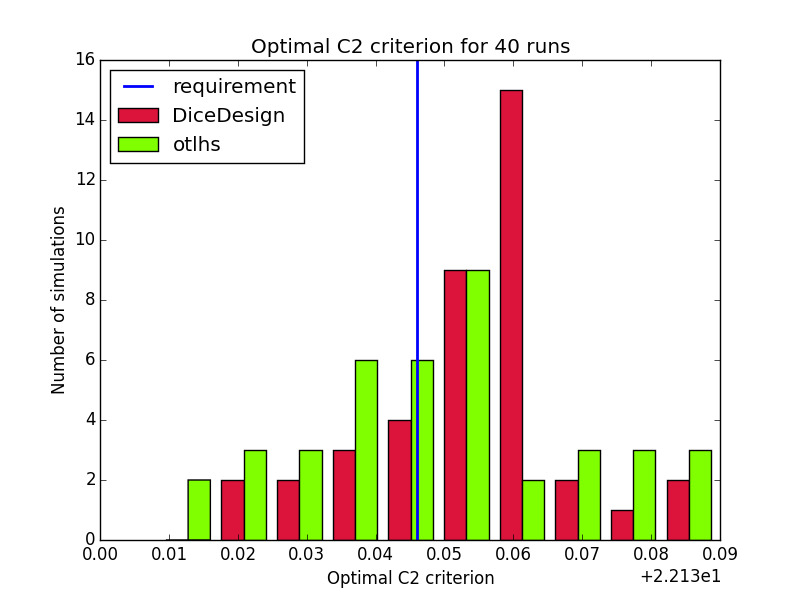
\includegraphics[scale=0.4]{comp_c2_large.png} & 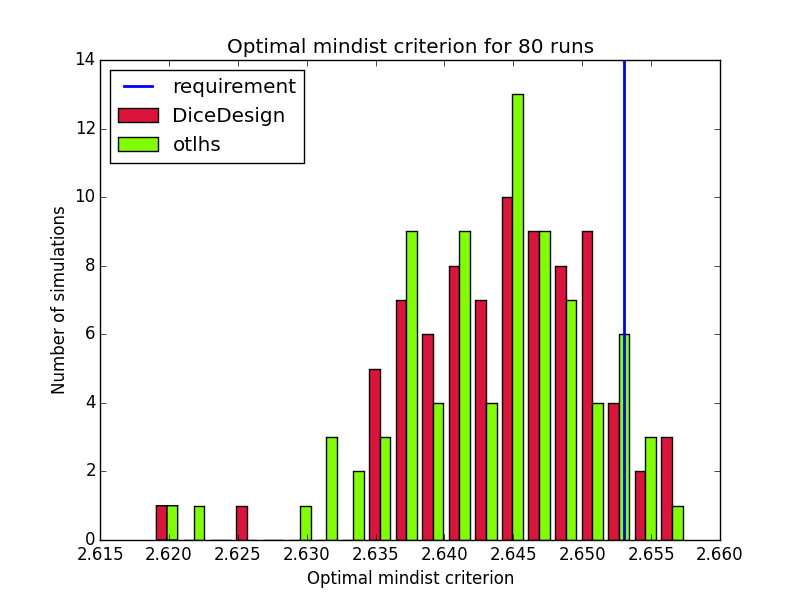
\includegraphics[scale=0.4]{comp_mindist_large.png}\\
 Comparison on 40 runs for test id 3 & Comparison on 80 runs for test id 4\\
\end{tabular}
\end{center}
\caption{Results comparison with restarts}
\label{comp_otlhs_dicedesign_tests}
\end{figure}

In addition, designs, optimized criterion convergence and elementary perturbation probability are given in figures \ref{results_sa_test_id1}, \ref{results_sa_test_id2} and \ref{results_sa_test_id34} (for dimension $50$, only criterion history is displayed).
\begin{figure}[!h]
\begin{center}
\begin{tabular}{>{\centering\arraybackslash}m{8cm}>{\centering\arraybackslash}m{8cm}}
 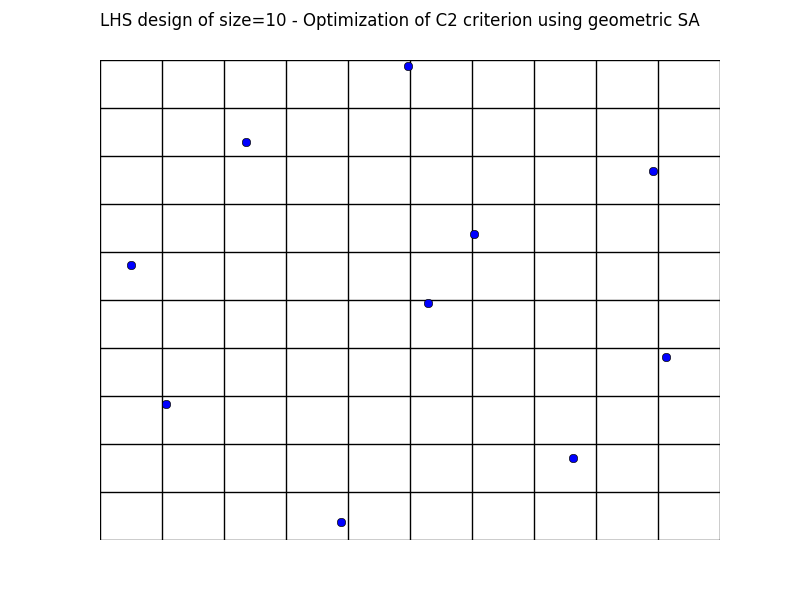
\includegraphics[scale=0.35]{lhs_sa_geom_10.png} & 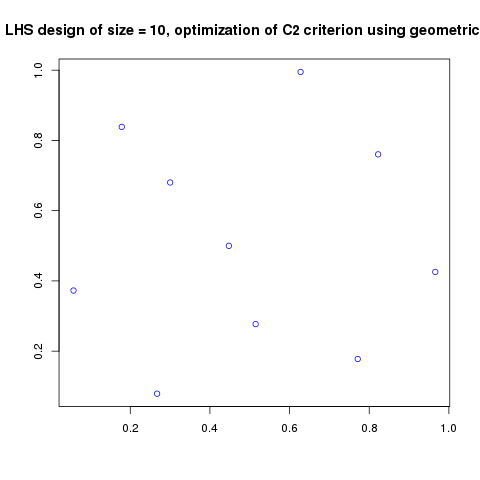
\includegraphics[scale=0.35]{dice_lhs_sa_geom_10.png} \\
 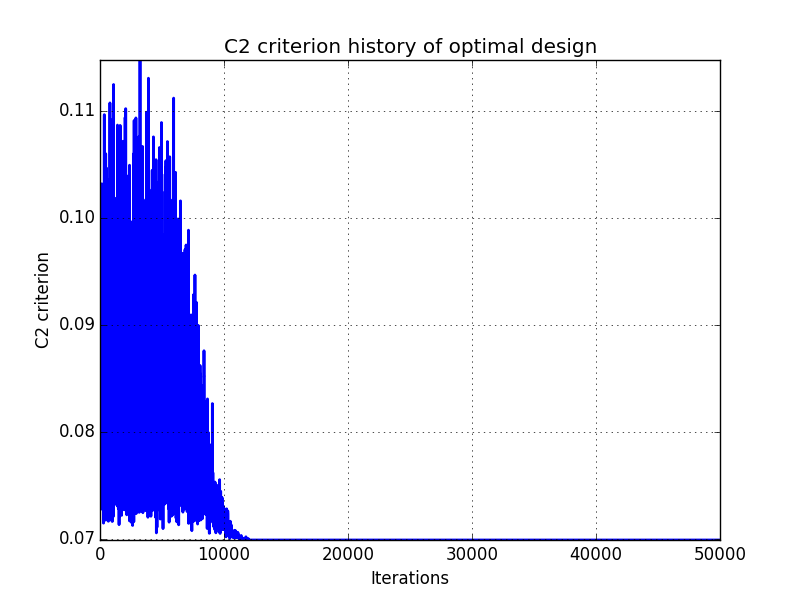
\includegraphics[scale=0.35]{crit_sa_geom.png}   & 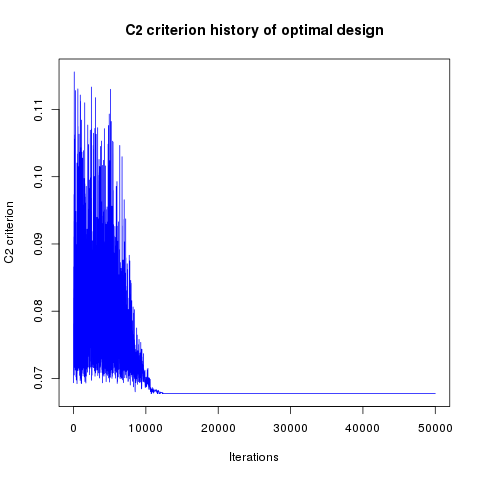
\includegraphics[scale=0.35]{dice_c2_crit.png}   \\
 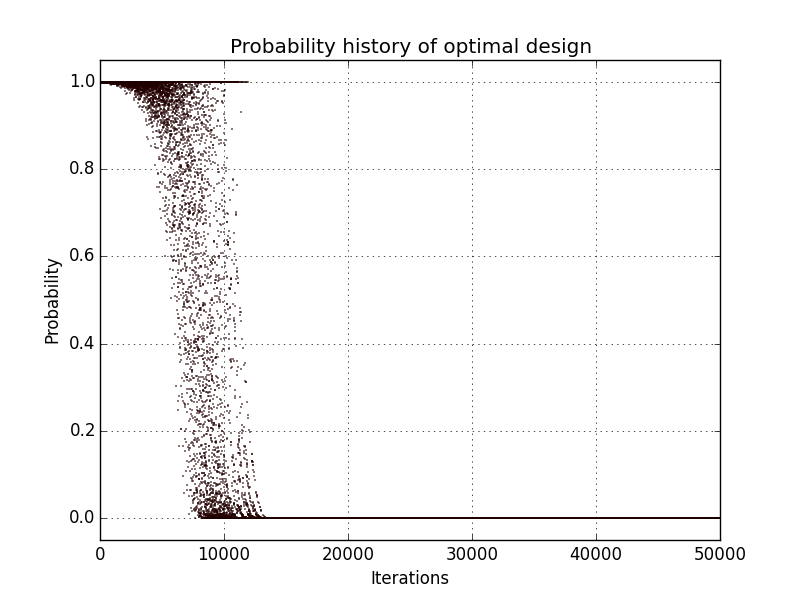
\includegraphics[scale=0.35]{lhs_c2_proba.png}   & 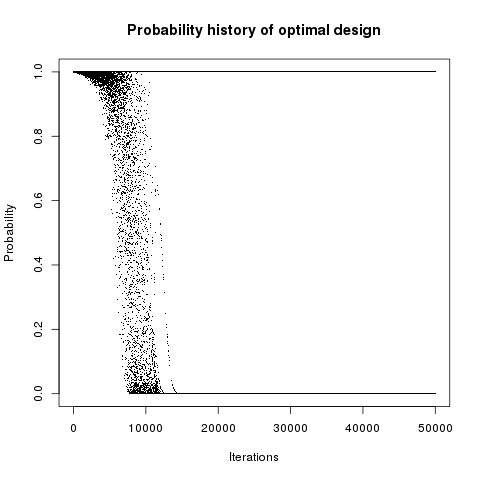
\includegraphics[scale=0.35]{dice_c2_proba.png}\\
 \texttt{otlhs} & \texttt{DiceDesign}
\end{tabular}
\end{center}
\caption{Simulated annealing results - Test id 1}
\label{results_sa_test_id1}
\end{figure}

\begin{figure}[!h]
\begin{center}
\begin{tabular}{>{\centering\arraybackslash}m{8cm}>{\centering\arraybackslash}m{8cm}}
 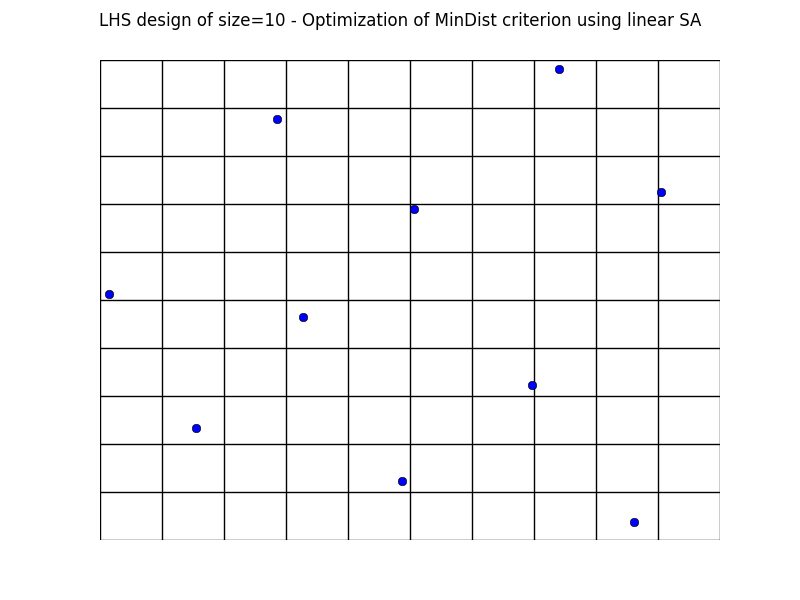
\includegraphics[scale=0.35]{lhs_sa_lin_10.png} & 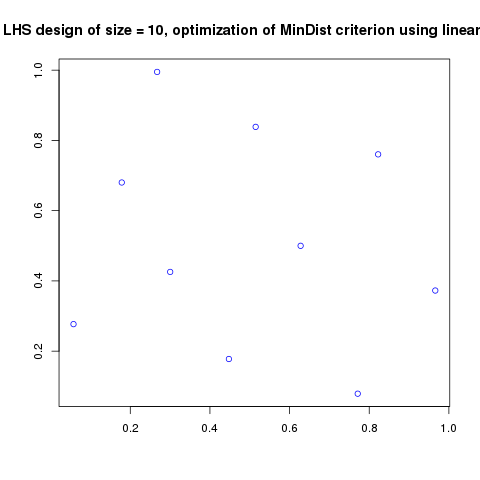
\includegraphics[scale=0.35]{dice_lhs_sa_lin_10.png}\\
 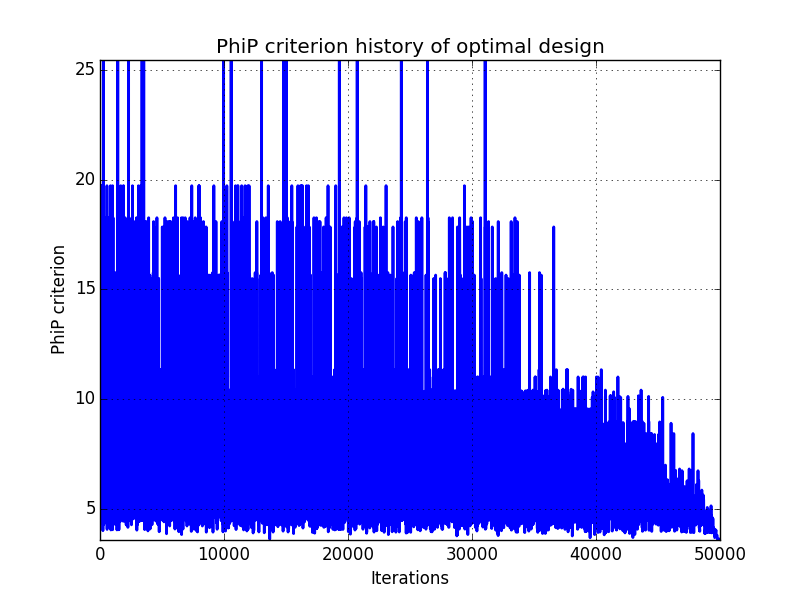
\includegraphics[scale=0.35]{crit_sa_lin.png}   & 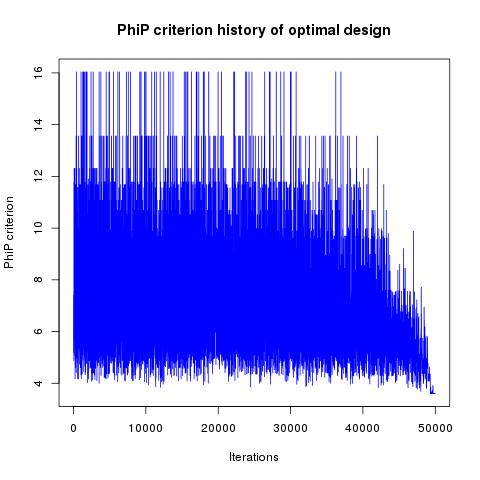
\includegraphics[scale=0.35]{dice_mindist_crit.png}\\
 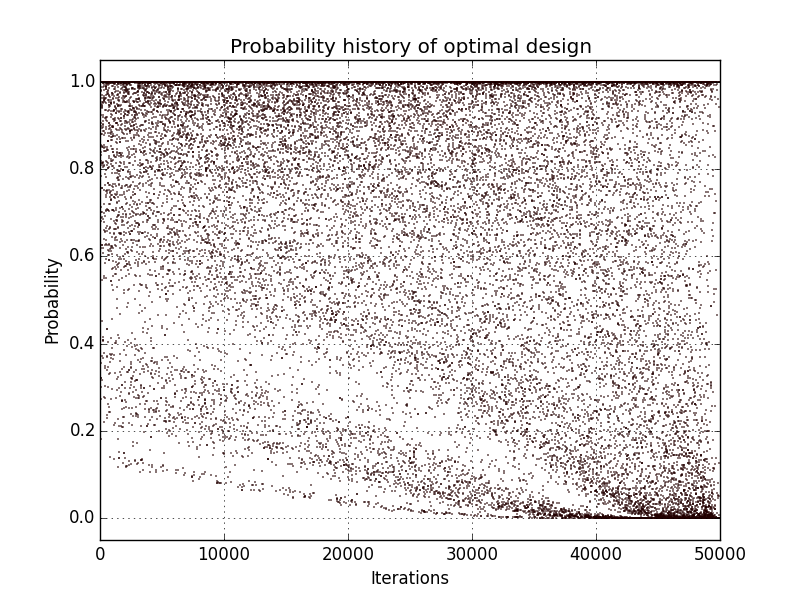
\includegraphics[scale=0.35]{lhs_mindist_proba.png}   & 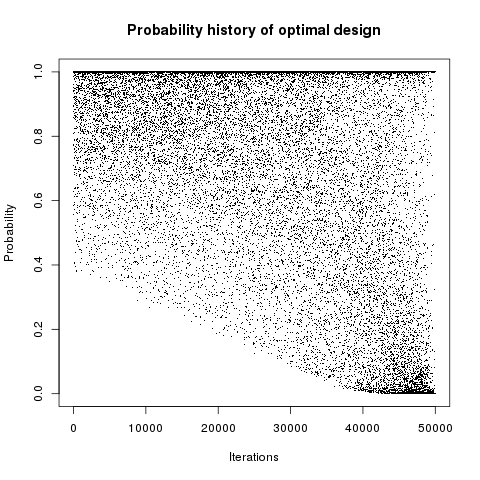
\includegraphics[scale=0.35]{dice_mindist_proba.png}\\
 \texttt{otlhs} & \texttt{DiceDesign}
\end{tabular}
\end{center}
\caption{Simulated annealing results - Test id 2}
\label{results_sa_test_id2}
\end{figure}

\begin{figure}[!h]
\begin{center}
\begin{tabular}{>{\centering\arraybackslash}m{8cm}>{\centering\arraybackslash}m{8cm}}
 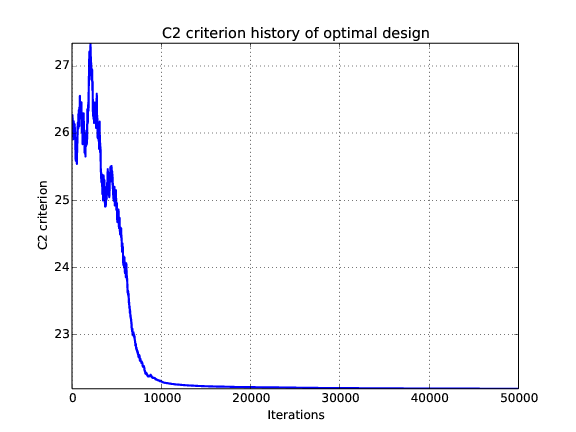
\includegraphics[scale=0.35]{otlhs_c2_crit_big.png} & 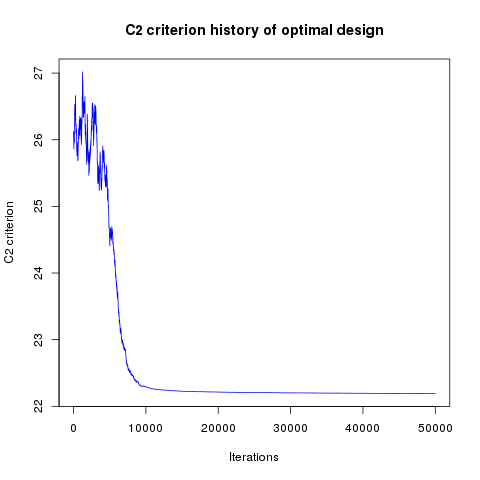
\includegraphics[scale=0.35]{dice_c2_crit_big.png}\\
 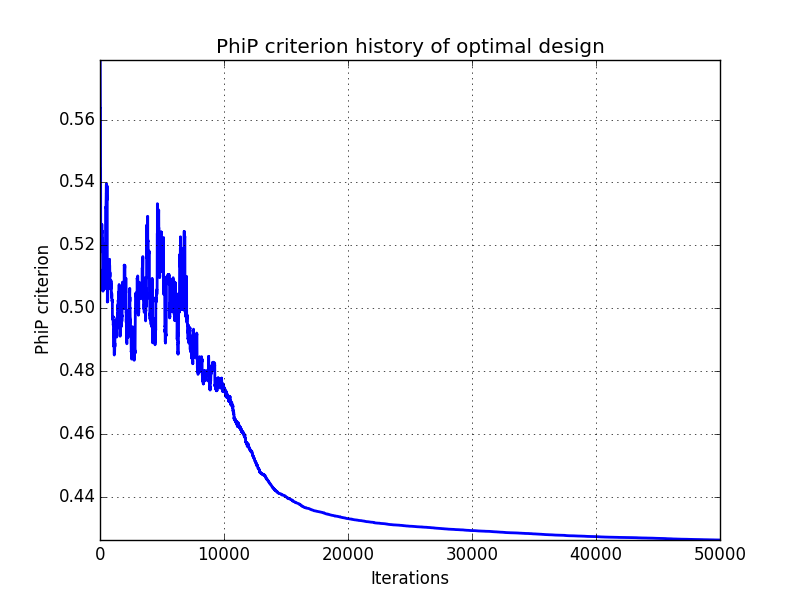
\includegraphics[scale=0.35]{otlhs_mindist_crit_big.png}   & 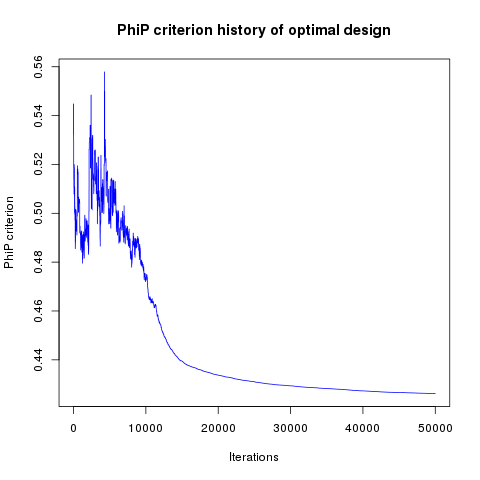
\includegraphics[scale=0.35]{dice_mindist_crit_big.png}\\
\end{tabular}
\end{center}
\caption{Simulated annealing criterion results - Test id 3 and 4}
\label{results_sa_test_id34}
\end{figure}
Results are very similar between the two implementations.  It must be noted that there are many plots with probability~1.  The reason is that DiceDesign accepts both row indices to be equal when checking for elementary perturbations.


